%!TEX TS-program = pdflatex
%!TEX encoding = utf8
\documentclass[12pt, oneside]{book}
\usepackage[T1]{fontenc}
\usepackage[utf8]{inputenc}
\usepackage[english]{babel}
%% FONTS: libertine+biolinum+stix
\usepackage[mono=false]{libertine}
\usepackage[notext]{stix}
\usepackage{hyperref}
\addto{\captionsenglish}{%
  \renewcommand{\bibname}{References}
}

% =====================
% = Datos importantes =
% =====================
% hay que rellenar estos datos y luego
% ir a \begin{document}

\title{Uncertainty treatment in Maxwell equations' resolution using the FDTD method.}
\author{Alberto Prados Pérez}
\date{9 de Julio de 2021}
\newcommand{\tutores}[1]{\newcommand{\guardatutores}{#1}}
\tutores{Dr. Luis Manuel Díaz Angulo \\
		 Dr. Miguel David Ruiz Cabello}

% ======================
% = Páginas de títulos =
% ======================
\makeatletter
\edef\maintitle{\@title}
\renewcommand\maketitle{%
  \begin{titlepage}
      \vspace*{1.5cm}
      \parskip=0pt
      \Huge\bfseries
      \begin{center}
          \leavevmode\includegraphics[totalheight=6cm]{sello.jpg}\\[2cm]
          \@title
      \end{center}
      \vspace{1cm}
      \begin{center}
          \@author
      \end{center}
      
  \end{titlepage}
  
  \begin{titlepage}
  \parindent=0pt
  \begin{flushleft}
  \vspace*{1.5mm}
  \setlength\baselineskip{0pt}
  \setlength\parskip{0mm}
  \begin{center}
      \leavevmode\includegraphics[totalheight=4.5cm]{sello.jpg}
  \end{center}
  \end{flushleft}
  \vspace{1cm}
  \bgroup
  \Large \bfseries
  \begin{center}
  \@title
  \end{center}
  \egroup
  \vspace*{.5cm}
  \begin{center}
  \@author
  \end{center}
  \vspace{0.5cm}
  \begin{center}
  \@date
  \end{center}
  \vspace*{1.8cm}
  \begin{flushright}
  \begin{minipage}{8.45cm}
      Memoria del {\bf Trabajo Fin de Máster}.\\ 
      Máster en Física y Matemáticas (FisyMat) \\ 
      University of Granada.

      \vspace*{7.5mm}

      Tutored by:
      % \vspace*{5mm}
  \end{minipage}\par
  \begin{tabularx}{8.45cm}[b]{@{}l}
      \guardatutores
  \end{tabularx}
   \end{flushright}
      \vspace*{\fill}
   \end{titlepage}
   %%% Esto es necesario...
   \pagestyle{tfg}
   \renewcommand{\chaptermark}[1]{\markright{\thechapter.\space ##1}}
   \renewcommand{\sectionmark}[1]{}
   \renewcommand{\subsectionmark}[1]{}
  }
\makeatother

% ======================================
% = Color de la Universidad de Sevilla =
% ======================================
\usepackage{tikz}
\definecolor{USred}{cmyk}{0,1.00,0.65,0.34}

% =========
% = Otros =
% =========
\usepackage[]{tabularx}
\usepackage[]{enumitem}
\setlist{noitemsep}

% ==========================
% = Matemáticas y teoremas =
% ==========================
\usepackage[]{amsmath}
\usepackage[]{amsthm}
\usepackage[]{mathtools}
\usepackage[]{bm}
\usepackage[]{thmtools}
\usepackage{braket}
\usepackage{accents}
\newcommand{\ubar}[1]{\underaccent{\bar}{#1}}

\newcommand{\marcador}{\vrule height 10pt depth 2pt width 2pt \hskip .5em\relax}
\newcommand{\cabeceraespecial}{%
    \color{USred}%
    \normalfont\bfseries}
\declaretheoremstyle[
    spaceabove=\medskipamount,
    spacebelow=\medskipamount,
    headfont=\cabeceraespecial\marcador,
    notefont=\cabeceraespecial,
    notebraces={(}{)},
    bodyfont=\normalfont\itshape,
    postheadspace=1em,
    numberwithin=chapter,
    headindent=0pt,
    headpunct={.}
    ]{importante}
\declaretheoremstyle[
    spaceabove=\medskipamount,
    spacebelow=\medskipamount,
    headfont=\normalfont\itshape\color{USred},
    notefont=\normalfont,
    notebraces={(}{)},
    bodyfont=\normalfont,
    postheadspace=1em,
    numberwithin=chapter,
    headindent=0pt,
    headpunct={.}
    ]{normal}
\declaretheoremstyle[
    spaceabove=\medskipamount,
    spacebelow=\medskipamount,
    headfont=\normalfont\itshape\color{USred},
    notefont=\normalfont,
    notebraces={(}{)},
    bodyfont=\normalfont,
    postheadspace=1em,
    headindent=0pt,
    headpunct={.},
    numbered=no,
    qed=\color{USred}\marcador
    ]{demostracion}

% Los nombres de los enunciados. Añade los que necesites.
\declaretheorem[name=Observaci\'on, style=normal]{remark}
\declaretheorem[name=Corolario, style=normal]{corollary}
\declaretheorem[name=Proposici\'on, style=normal]{proposition}
\declaretheorem[name=Lema, style=normal]{lemma}

\declaretheorem[name=Teorema, style=importante]{theorem}
\declaretheorem[name=Definici\'on, style=importante]{definition}

\let\proof=\undefined
\declaretheorem[name=Demostraci\'on, style=demostracion]{proof}


% ============================
% = Composición de la página =
% ============================
\usepackage[
    a4paper,
    textwidth=80ex,
]{geometry}

\linespread{1.069}
\parskip=10pt plus 1pt minus .5pt
\frenchspacing
% \raggedright


% ==============================
% = Composición de los títulos =
% ==============================

\usepackage[explicit]{titlesec}

\newcommand{\hsp}{\hspace{20pt}}
\titleformat{\chapter}[hang]
    {\Huge\sffamily\bfseries}
    {\thechapter\hsp\textcolor{USred}{\vrule width 2pt}\hsp}{0pt}
    {#1}
\titleformat{\section}
  {\normalfont\Large\sffamily\bfseries}{\thesection\space\space}
  {1ex}
  {#1}
\titleformat{\subsection}
  {\normalfont\large\sffamily}{\thesubsection\space\space}
  {1ex}
  {#1}

% =======================
% = Cabeceras de página =
% =======================
\usepackage[]{fancyhdr}
\usepackage[]{emptypage}
\fancypagestyle{plain}{%
    \fancyhf{}%
    \renewcommand{\headrulewidth}{0pt}
    \renewcommand{\footrulewidth}{0pt}
}
\fancypagestyle{tfg}{%
    \fancyhf{}%
    \renewcommand{\headrulewidth}{0pt}
    \renewcommand{\footrulewidth}{0pt}
    \fancyhead[LE]{{\normalsize\color{USred}\bfseries\thepage}\quad
                    \small\textsc{\MakeLowercase{\maintitle}}}
    \fancyhead[RO]{\small\textsc{\MakeLowercase{\rightmark}}%
                    \quad{\normalsize\bfseries\color{USred}\thepage}}%
                    }

% =============================
% = El documento empieza aquí =
% =============================
\begin{document}


\maketitle

\frontmatter
\tableofcontents

\mainmatter

%========================
\chapter*{English Abstract}
\addcontentsline{toc}{chapter}{English Abstract}
\markright{English Abstract}



\begin{otherlanguage}{english}
In this work an analysis of different methods to treat uncertainties of the electrical parameters of materials is presented in the context of Maxwell's equations in the time domain. In various frameworks, including, for example, the interaction of electric fields with biological tissues, the need to know the variance and other statistical quantities of the electric or magnetic fields may be of interest. The remainder of this work is organized as follows. \\
\indent First of all, the Finite Difference Time Domain (FDTD) method is presented and a short review is done emphasizing the important aspects of the algorithm that have been found in the development of the code implemented to do the simulations. \\
\indent Then, a section is devoted to the reflection and transmission coefficients, which will be used to test the different approaches to compute the uncertainties. \\
\indent Next, the Stochastic Finite Difference Time Domain (S-FDTD) formalism is implemented as well. This method obtains the variance of the fields in addition to the average values, which are the same as for the FDTD method. This is performed updating the standard deviations of the electric and magnetic fields in time in an analogous way as is done in the FDTD method for the fields. However, those results are not exact since the update equations for the standard deviation use the correlations coefficients between the electrical parameters and the fields which, in principle, are unknown, and some approximations will be needed. \\
\indent Lastly, the Monte Carlo method is carried out. This method is implemented in two different ways. The first one consider the materials treated in the simulation as a whole, for that reason, just two electrical parameters, namely the permittivity and conductivity of the material, are randomly generated in each simulation. The second one treats the material ``cell by cell" and the number of randomly generated parameters will depend on the thickness of the material.
One of the goals sought with these two implementations is to better understand the sources of uncertainty. The results obtained with the Monte Carlo methodd will also be compared with those obtained with the S-FDTD formalism. 
\end{otherlanguage}

\chapter*{Resumen en Español}
\addcontentsline{toc}{chapter}{Resumen en Español}
\markright{Resumen en Español}

\begin{otherlanguage}{spanish}
En este trabajo se presenta un análisis de varios métodos para el tratamiento de las incertidumbres de los parámetros eléctricos en las ecuaciones de Maxwell en el dominio del tiempo. En distintas áreas, como por ejemplo, el análisis de tejidos biológicos, es necesario conocer algunas cantidades estadísticas como son la varianza, además de los valores medios. \\
\indent El primer paso será presentar el método de las diferencias finitas en el dominio del tiempo (FDTD), donde se hará énfasis en los aspectos importantes del algoritmo que se han encontrado durante el desarrollo del código implementado para llevar a cabo las simulaciones. \\
\indent A continución se dedica una sección para introducir dos cantidades que han sido relevantes para la comprobación de los métodos utilizados, se trata de la reflectancia y la transmitancia. \\
\indent Después de esto se desarrolla el formalismo de las diferencias finitas en el dominio del tiempo estocástico (S-FDTD). Este nos permitirá obtener la varianza de los campos, además de los valores medios, que coinciden con los que proporciona el método FDTD. Este método sigue un esquema similar al FDTD, al que se añaden dos ecuaciones correspondientes a las desviaciones típicas de los campos. Sin embargo, este último no es exacto, en las ecuaciones para las desviaciones típicas aparecen los coeficientes de correlación entre los parámetros eléctricos y los campos y, en principio, no tenemos información acerca de ellos y algunas aproximaciones serán necesarias. \\
\indent Por último, el método Monte Carlo es implementado de dos formas distintas. La primera considera cada material como un solo ente, y por tanto, en cada simulación Monte Carlo se generan únicamente dos parámetros aleatorios, el correspondiente para la permitividad y para la conductividad. La segunda forma considera los materiales ``punto a punto", y el número de parámetros aleatorios dependerá del grosor del material. Con esto se busca entender las posibles causas de las incertidumbres. Además , el método Monte Carlo se utilizará para realizar una comparación con los resultados del método S-FDTD.

\end{otherlanguage}


\chapter{Introduction}
In this work an analysis of the Stochastic Finite-Difference Time-Domain (S-FDTD) method is presented \cite{smith2011stochastic,smith2012stochastic}. The S-FDTD method is an approach for computing the variance in the propagation of electromagnetic fields that arises due to uncertainties in electrical properties. Those may vary because of uncertainty in the measurements, variations in materials, variations in manufacturing, etc. \\
\indent The traditional FDTD method \cite{taflove2005computational} uses electrical properties such as permittivity and conductivity as inputs and returns the average values of the fields. So, if our goal is to compute other statistical quantities such as the variance of the field, although other statistical properties may also be of interest such as $90\%$ confidence intervals, before the development of the S-FDTD we would be bound to use the Monte Carlo method \cite{Sadiku2009}. This implies running a huge number of simulations to obtain statistics for the fields, this can be made in one dimensional simulations but would be impractical for three dimensional ones.\\
\indent The S-FDTD technique takes the same two equations of the FDTD method as a starting point, namely the discretized version of Faraday's and Ampere's law. Next, the delta method \cite{casella2021statistical}, which can be seen as a Taylor's expansion, is used to derive expressions for the mean and variance values. The mean values for this method are the same as those obtained with the FDTD as expected; to get this, higher order terms are neglected in the expansion. For the variance, a series of approximations are made as well, and the procedure is much more complex. At the end of the method two expressions are derived for the electric and magnetic field. In this expressions appear some unknown quantities, those are the correlation coefficients between the electrical properties with the fields. \\
\indent The main goal of this work is to explore these correlations. In principle we can not know anything else beyond that they must be bounded between $-1$ and $1$. These coefficients vary with time and a model to try to find them in each time step have not been proposed and this question is still an open problem. Until now, several approximations have been tried in order to estimate the correlation coefficients \cite{Zygiridis2017}, for example, assuming a value of one, which overestimates the result given by the Monte Carlo method. Therefore, this work will seek to understand the nature of this correlations which could be the first step to propose an accurate method to compute these coefficients. \\
\indent The applications of the S-FDTD method is quite broad. There are a lot of areas in which the FDTD method is applied that vary statistically, and in which an evaluation of the statistical properties of the fields may be needed. For example, the FDTD method is used in bioelectromagnetics \cite{gandhi1996electromagnetic,furse1996fdtd,Christ2005}, geophysical prospecting \cite{johnson2001cross} or atmospheric studies \cite{simpson2007review}.

\section{Objectives.}

The main objective of this work is to develop a code written in Python that allows us to simulate the propagation of electric fields through materials, computing both the mean value and variance of those fields. To do this, first, the FDTD method is going to be established and validated using the analytical result for the reflectance and transmittance of a slab of material. \\
\indent After that, the next goal is to include the S-FDTD method which will allow to compute the variance of the fields.
Most of the analysis will use the reflectance and transmittance of a slab of material. The latter results will be compared with analytical ones whenever it is possible. \\
\indent The next step is to develop the same computations with the Monte Carlo method. This method is considered to be the most accurate, but it has much more computational cost. For this reason, the results obtained through this method will be used to compare the ones obtained with S-FDTD analysis. Lastly, two ways of implementing the Monte Carlo will be discussed,  trying to understand with this the different sources of uncertainty and the correlation of the variables involved in the FDTD scheme.
\indent The files containing the code are of public access, released with license GPL3, and can be found in the next link of Github: \url{https://github.com/Alber6/TFM}.


\chapter{Maxwell's equations and the Yee algorithm.}

In this section, an introduction to the FDTD algorithm is provided \cite{yee1966numerical}. The formalism treated here will be the one dimensional case. First, the free space case will be covered in detail, and then some complexity will be introduced until the case for a lossy dielectric medium is reached. The following discussion of this work will be done in those media.

\section{Introduction to the finite differences.}
The central finite differences \cite{li2017numerical} constitute the core of the FDTD algorithm, and for that reason an introduction is given here. The tool used to derive the expression for the forward, backward and central finite difference is the Taylor expansion. Since we are concerned with Maxwell's equations, we are only interested in the first derivative although higher order derivatives can be computed. 
The formulas for the forward and backward differences are:
\begin{equation}
\Delta_{+h} f(x)= f(x+h) - f(x),
\end{equation}
\begin{equation}
\Delta_{-h} f(x)= f(x) - f(x-h).
\end{equation}
These two forms for the differences approximate the derivative with an error proportional to $h$. However, the central finite difference gives an error proportional to $h^2$, and this is the one used to discretize Maxwell's equations later. To find this expression, Taylor's expansion is going to be employed with $h=\Delta x /2$:
\begin{equation}
\begin{aligned}
f\left(x+\frac{\Delta x}{2}\right)=f(x)+f'(x)\frac{\Delta x}{2}+ \frac{1}{2} f''(x)\left( \frac{\Delta x}{2} \right)^2 + \mathcal{O}\left(h^{2}\right), \\
f\left(x-\frac{\Delta x}{2}\right)=f(x)-f'(x)\frac{\Delta x}{2}+ \frac{1}{2} f''(x)\left( \frac{\Delta x}{2} \right)^2 + \mathcal{O}\left(h^{2}\right),
\end{aligned}
\end{equation}
and thus, subtracting the two equations, we obtain:
\begin{equation}
\delta f(x)= \frac{f\left(x+\frac{\Delta x}{2}\right)-f\left(x-\frac{\Delta x}{2}\right)}{\Delta x}.
\end{equation}
This equation will be used both for the spatial and time derivatives that one finds in Maxwell's equations.


\section{One dimensional Maxwell's equations.}
From the Maxwell's curl equations for free space
\begin{equation}
\begin{aligned}
&\frac{\partial E}{\partial t}=\frac{1}{\varepsilon_{0}} \nabla \times \boldsymbol{H}, \\
&\frac{\partial \boldsymbol{H}}{\partial t}=-\frac{1}{\mu_{0}} \nabla \times \boldsymbol{E},
\end{aligned}
\end{equation}
we can obtain the one dimensional ones which are reduced to:

\begin{align}
& \frac{\partial E_x}{\partial t}=-\frac{1}{\epsilon_0}  \frac{\partial H_y}{\partial z}, \\
& \frac{\partial H_y}{\partial t}=-\frac{1}{\mu_0} \frac{\partial E_x}{\partial z}.
\end{align}

\noindent These equations are those of a plane wave propagating in the $z$ direction with the electric field in the $x$ direction and the magnetic field oriented in the $y$ direction. Using the central difference approximation in the spatial and time derivatives, the following form of the equations is obtained \cite{yee1966numerical,taflove2005computational}:

\begin{align}
 \frac{E_x^{n+\frac{1}{2}}(k)-E_x^{n-\frac{1}{2}}(k)}{\Delta t}=-\frac{1}{\epsilon_0}\frac{H_y^n \left(k+\frac{1}{2}\right) - H_y^n\left(k-\frac{1}{2}\right)}{\Delta z}, \\
\frac{H_y^{n+1} \left(k+\frac{1}{2}\right) -H_y^{n}\left( k +\frac{1}{2}\right)}{\Delta t}=-\frac{1}{\mu_0}\frac{E_x^{n+\frac{1}{2}} \left(k+1\right) - E_x^{n+\frac{1}{2}}\left(k\right)}{\Delta z}.
\end{align}
In these equations, the superscript indicates the time step such that time is $t=\Delta t \cdot n$. The terms in parenthesis represent the spatial position, the discretized elements of space are called cells. The fundamental idea of the algorithm is then to update the fields, for example, to get the electric field at the next time step we need to know the electric field in the previous time step and the two adjacent and previous magnetic fields. This can be easily seen rearranging the last equations:
\begin{equation}\label{updateequationseandh}
\begin{gathered}
E_{x}^{n+1 / 2}(k)=E_{x}^{n-1 / 2}(k)-\frac{\Delta t}{\varepsilon_{0} \cdot \Delta z}\left[H_{y}^{n}\left(k+\frac{1}{2}\right)-H_{y}^{n}\left(k-\frac{1}{2}\right)\right], \\
H_{y}^{n+1}\left(k+\frac{1}{2}\right)=H_{y}^{n}\left(k+\frac{1}{2}\right)-\frac{\Delta t}{\mu_{0} \cdot \Delta z}\left[E_{x}^{n+1 / 2}(k+1)-E_{x}^{n+1 / 2}(k)\right].
\end{gathered}
\end{equation}
The algorithm is interleaving the two fields both in space and time. It is important to realize that, in order to code the algorithm, the array associated to the magnetic field, which is one dimensional, will have one less element. The first and last positions of the array corresponding to the electric field will not be modified with the last equations but with the absorbing boundary conditions, which will be explained in the next section. Hence, the basics of the algorithm have been discussed already, it can be summed up to iterate the computation of the electric field, then the magnetic one and repeat this process until the simulation time is finished. \\
\indent The Maxwell's equations are almost symmetric, the only thing breaking that symmetry is the difference in the electrical parameters, namely the permittivity and permeability. This will make the fields differ by several orders of magnitude which may cause some problems at the time of coding the algorithm. This problem can be solved in various ways, for example, working with dimensions in which the value of those parameters in one. However, in this work another approach is followed, which seems to be more intuitive to understand some of the results obtained. The selected approach consists in changing the electric field with the following change of variables \cite{houle2020electromagnetic}:
\begin{equation}\label{changeofvariable}
\tilde{E}=\sqrt{\frac{\epsilon_0}{\mu_0}} E.
\end{equation}
The tilde in the electric field will be dropped for simplicity. Now, the boundary conditions are discussed.

\subsection{Absorbing boundary conditions.}
The Mur's absorbing boundary conditions \cite{mur1981absorbing} are the selected ones in this work. These conditions allow the fields to exit the mesh as it if continued infinitely, i.e. the fields will not be reflected back, it is like they are being absorbed. At the boundaries of the mesh we can not apply the previous equation for the update of the electric field since we do not have one of the magnetic fields required. The equations that enable us to compute the electric field at those positions are:
\begin{equation}\label{boundarycondition1}
E_{x}^{n+1 / 2}(0)=E_{x}^{n-1 / 2}(1)+\frac{c \Delta t-\Delta x}{c \Delta t+\Delta x}\left(E_{x}^{n+1 / 2}(1)-E_{x}^{n-1 / 2}(0)\right),
\end{equation}
and we know every field in the right hand side of the equation since $E_{x}^{n+1 / 2}(1)$ have been already computed using the update equation \ref{updateequationseandh}. In the last equation $c$ is just the speed of light in a vacuum. For the boundary at the right of the mesh the equation is analogous to this one:
\begin{equation}\label{boundarycondition2}
E_{x}^{n+1 / 2}(N)=E_{x}^{n-1 / 2}(N-1)+\frac{c \Delta t-\Delta x}{c \Delta t+\Delta x}\left(E_{x}^{n+1 / 2}(N-1)-E_{x}^{n-1 / 2}(N)\right),
\end{equation}
with $N$ being the number of cells in the mesh.


\subsection{Stability and cell size in the FDTD method.}
In the previous equations appear the spatial step and time step. Those two parameters can not be selected at random as there is one constraint \cite{taflove2005computational}, namely the Courant condition. The fields can not go faster than light and the equations have to respect causality. To propagate through one cell requires a minimum amount of time $\Delta t= \Delta x/c$. In this work the following relation has been selected to obtain the time step from the spatial one:
\begin{equation}
\Delta t= \frac{\Delta x}{2c}.
\end{equation}
\indent Now, it only remains to determine cell size or spatial step. The size of the cells and the number of it must be enough to resolve the fields propagating through them. A rule to follow is to have $10$ cells per wavelength. So to determine it, we should look at the frequency we are working with and them estimate the wavelength in the material with highest dielectric constant, as it will be the shortest wavelength to resolve. In the case treated in next sections \cite{smith2012stochastic}, biological tissues are being simulated and the muscle is the one with a highest dielectric constant. Using this, the shortest wavelength is found and it is then divided by $40$.


\subsection{Sources.}
There are two main ways of establishing the source \cite{taflove2005computational,Mansourabadi2008}. They are called hard source and soft source. The hard source will act like a perfect conductor in the point of the mesh where it is defined. This means that the fields will be completely reflected and this prevents most of the analysis of this work. To implement a hard source, one just imposes the required value in the desired cell of the mesh. In the other hand, the soft source allow the fields to propagate through, hence, the fields will reach the boundaries and will be absorbed. Implementing this kind of source is also easy, just add the source term to the field in the selected point. The sources used in the next sections are 
a Gaussian pulse and a sinusoidal plane given by the following equations (in pseudocode format):
\begin{equation}
\text{pulse} = \exp( -0.5 *( ( \text{t}_0 - \text{t}) / \text{s}_0 )**2),
\end{equation}

\begin{equation}
\text{pulse} = \sin(2*\text{pi}*\text{freq}*\text{dt}*\text{time}-\text{step}).
\end{equation}


\section{Propagation in a lossy dielectric medium.}
To simulate the propagation in a dielectric medium we just need to add the relative permittivity to the update equation. However, now a simulation in media with conductivity is sought. The loss term will attenuate the propagation of energy. Writing Maxwell's curl equations again including those terms we get:
\begin{equation}\label{maxwelllossymedium}
\begin{aligned}
\varepsilon_{r} \varepsilon_{0} \frac{\partial E}{\partial t} &=\nabla \times H-J, \\
\frac{\partial H}{\partial t} &=-\frac{1}{\mu_{0}} \nabla \times E,
\end{aligned}
\end{equation}
where the current density can be expressed in the following way $J=\sigma E$. Introducing this in the last equation and rearranging to get an update equation, the following expression is obtained for a lossy dielectric medium \cite{taflove2005computational}:
\begin{equation}\label{updateequationlossymedium}
E_{x}^{n+1/2}(k)  = \frac{\left(\frac{\varepsilon_{r} \varepsilon_{o}}{\Delta t}-\frac{\sigma}{2}\right)}{\left(\frac{\varepsilon_{r} \varepsilon_{o}}{\Delta t}+\frac{\sigma}{2}\right)} E_{x}^{n-1/2}(k) 
- \frac{\left[H_{y}^{n}(k+1 / 2)-H_{y}^{n}(k-1 / 2)\right]}{\left(\frac{\varepsilon_{r} \varepsilon_{o}}{\Delta t}+\frac{\sigma}{2}\right) \Delta z} .
\end{equation}
To get this expression, the only thing we did not have is the electric field at time step $n$ which appears in the current density term. As we do not compute those values in our algorithm an approximation is made to estimate them. The values of the fields $E_x^n$ are the arithmetic average of the values of the fields at time steps $E_x^{n+1/2}$ and $E_x^{n-1/2}$:
\begin{equation}
E_x^n(k)=\frac{E_x^{n+1/2}(k)+E_x^{n-1/2}(k)}{2}.
\end{equation}
\indent Therefore, from now on equation \ref{updateequationlossymedium} will be used to simulate the materials. For each layer of a different material in the mesh it suffices to change the coefficients of the fields in  the update equation according to the material properties.


\chapter{Reflectance and Transmittance.}
This section is devoted to present two quantities that will be computed in order to compare the different methods used to obtain the uncertainties of the fields. These quantities are the power reflection and transmission coefficients, also known as the reflectance and transmittance \cite{orfanidis2002electromagnetic}. Both give the percentage of incident power which is reflected and transmitted respectively. 

\section{Introduction to the coefficients.}
\indent First, consider a single dielectric slab (see Figure \ref{dielectricslab}) and a normal incident field coming from the left such that to the right of the slab there is only a forward wave. If this slab is in free space, then the elementary reflection and transmission coefficients in the two interfaces are given by the following expressions: 
\begin{equation}
\rho_{1}=\frac{\eta_{1}-\eta_{0}}{\eta_{1}+\eta_{0}}, \quad \rho_{2}=\frac{\eta_{0}-\eta_{1}}{\eta_{0}+\eta_{1}}, \quad \tau_{1}=1+\rho_{1}, \quad \tau_{2}=1+\rho_{2}.
\end{equation}
with $\eta_0=\sqrt{\mu_0/\epsilon_0}$ and $\eta_1$ being the impedances of free space and the slab respectively. \\
\indent Starting from this, it is possible to determine the overall reflection coefficient, which is a function of frequency. Considering first a lossless medium, the reflection coefficient is  \cite{orfanidis2002electromagnetic}:
\begin{equation}
R(\omega)=\frac{\rho_{1}+\rho_{2} e^{-j \omega T}}{1+\rho_{1} \rho_{2} e^{-j \omega T}},
\end{equation}
where $\omega t= 2k_1 d$, $d$ is the thickness of the slab and $k_1=\omega/c_1$ is the propagation wave number ($j$ is the imaginary unit). $t$ is the two-way travel time delay through the slab. In an analogous way, it is possible to get the overall transmission coefficient. The expressions for these coefficients in terms of the fields are:
\begin{equation}
\begin{aligned}
& R=\frac{E_{1-}}{E_{1+}}, \\
&T=\frac{E_{2+}^{\prime}}{E_{1+}}.
\end{aligned}
\end{equation}
\indent The reflectance and transmittance of the slab is just the square modulus of these expressions. In the case of lossless media, energy conservation implies a relation between the two:
\begin{equation}\label{r2+t21}
\left|R\right|^{2} + |T|^{2}= 1.
\end{equation}
This equation is only valid if the medium to the left and to the right of the slab is the same one, as it is this case since the slab is in free space. Otherwise, the impedances of the two media will not cancel out and the correct expression would be the following one
\begin{equation}
1-\left|R\right|^{2}=\frac{\eta_{a}}{\eta_{b}}|T|^{2}.
\end{equation}
 
\begin{figure}\label{dielectricslab}
\centering
\includegraphics[scale=0.6]{dielectricslab.png}
\caption{Dielectric slab in free space. In the third medium there is only a forward wave. \cite{orfanidis2002electromagnetic}}
\end{figure}

\section{Analytical result.}
The formalism that allows us to compute these coefficients is referred as tansfer or transmission matrix. The transmission matrix is the combination of a $2\times 2$ matching matrix, which relates the forward and backward fields in the two sides of a determined interface, and a propagation matrix, which enables to get the fields in the next interface. The relation between the $E$ and $H$ fields ($E_+, E_-$ are just a combination of $E$ and $H$ given by Maxwell's equations) on one side and the other of the slab is given by
\begin{equation}
\left[\begin{array}{c}
E_{2} \\
H_{2}
\end{array}\right]=[\Phi]\left[\begin{array}{l}
E_{1} \\
H_{1}
\end{array}\right],
\end{equation}
where the transmission matrix, for homogeneous media is \cite{orfanidis2002electromagnetic}:
\begin{equation}\label{transmissionmatrix}
[\Phi]=\left[\begin{array}{cc}
\cosh (\gamma d) & \eta \sinh (\gamma d) \\
\eta^{-1} \sinh (\gamma d) & \cosh (\gamma d)
\end{array}\right],
\end{equation}
with $\gamma=j \omega \sqrt{\mu \varepsilon_{c}}$ being the material's complex propagation constant and $\varepsilon_{c}$ is the complex effective permittivity:
\begin{equation}
\varepsilon_{c}(\omega)=\varepsilon-j \frac{\sigma}{\omega}.
\end{equation}
\indent In case of having a collection of slabs of different homogeneous materials, then the transmission matrix is simply
\begin{equation}\label{variosmateriales}
[\Phi]=\prod_{i=1}^{N}\left[\Phi_{i}\right].
\end{equation}
\indent The last step is to conceptualize the slab as a two-port network in which each side of the slab is represented by a port and make use of the scattering matrix  \cite{orfanidis2002electromagnetic}
\begin{equation}\label{scatteringparameters}
[S]=\left[\begin{array}{ll}
S_{11} & S_{12} \\
S_{21} & S_{22}
\end{array}\right],
\end{equation}
which elements enables us to obtain the reflection and transmission coefficients with the next relations:
\begin{equation}
\begin{aligned}\label{rytcoef}
&|R|=\left|S_{11}\right|=\frac{\left|E_{1-}\right|}{\left|E_{1+}\right|}, \\
&|T|=\left|S_{21}\right|=\frac{\left|E'_{2+}\right|}{\left|E_{1+}\right|}.
\end{aligned}
\end{equation}
\indent Now, for slabs located in free space the coefficients can be obtained, if the incident electric field is a harmonic plane wave, as a function of the elements of the transmission matrix \ref{transmissionmatrix} since there is a relation between those and the scattering parameters \ref{scatteringparameters}, which is shown in the first table of \cite{frickey1994conversions}. The coefficients are:
\begin{equation}\label{analyticresultrt}
\begin{aligned}
&T=\frac{2 \eta_{0}}{\Phi_{11} \eta_{0}+\Phi_{12}+\Phi_{21} \eta_{0}^{2}+\Phi_{22} \eta_{0}}, \\
&R=\frac{\Phi_{11} \eta_{0}+\Phi_{12}-\Phi_{21} \eta_{0}^{2}-\Phi_{22} \eta_{0}}{\Phi_{11} \eta_{0}+\Phi_{12}+\Phi_{21} \eta_{0}^{2}+\Phi_{22} \eta_{0}}.
\end{aligned} 
\end{equation} 

\section{Reflectance and transmittance from the FDTD scheme.}\label{rytfromthesfdtdscheme}
The reflectance and transmittance have been computed using the outputs of the FDTD simulations. In order to do this, the values of the electric fields in a given position of the mesh, to the left of the slab for the reflectance and to the right for the transmittance, are stored in an array for all the time steps that the simulation lasts. It is important that the total simulation time is enough in order to incorporate the effect of most reflections that occur within the slab when the wave is reflected in both interfaces. \\
\indent The next step is to compute the Fourier transform of the fields since the previous expressions were written as a function of frequency, also the reflection and transmission response in the time domain is much more complex \cite{orfanidis2002electromagnetic}. This has been done using a Python module (NumPy) that incorporates the Fast Fourier Transform (FFT) function which is an algorithm for the Discrete Fourier Transform (DFT). \\
\indent Lastly, it is important to realize that the electric field stored in the array, at the point to the left of the slab, will be the sum of the reflected and incident ones, hence, the second one must be subtracted. Now, we can apply equations \ref{rytcoef} to obtain the reflection and transmission coefficients.




\chapter{Stochastic FDTD.}
\section{Introduction to the S-FDTD method.}
In the FDTD simulations considered in this work until this point, the values of the permittivity and conductivity used were the average values of the materials and therefore the values of the fields obtained were also their average values. However, materials are statistically variable and this have to be considered since the fields obtained will also vary statistically. \\
\indent As explained in the last paragraph \cite{smith2011stochastic,smith2012stochastic,Garcia2019}, a method is needed to compute these statistical quantities such as variance or standard variation.
The classical method used to compute the statistical properties is the Monte Carlo method, but this method comes under one big issue, it requires a huge number of simulations with properties selected at random.
Now, the Stochastic FDTD (S-FDTD) method is presented which provides a estimate of the mean and variation of the fields at every point in space and time. \\
\indent The usual FDTD equations are complemented with additional equations to compute the standard deviation, see Figure \ref{sfdtdalgorithmfigure}. Previously, the electrical properties $\epsilon_r$, $\ubar{\sigma}$ (where the symbol for conductivity has been changed to avoid confusion with the standard deviation) were the average values. \\
So the equations \ref{updateequationlossymedium} must be thought as stochastic equations with four random variables, namely $E_x$, $H_y$, $\epsilon_r$ and $\ubar{\sigma}$. \\
\indent The main problem we will encounter using this method is that the final equations for the standard deviation of the fields depends on the correlation coefficients of our variables, and we do not have an easy way to estimate or compute them. To make an estimation of these parameters some considerations can be taken into account, the typical procedure is to use another method, namely the Monte Carlo method, to give an estimation.

\begin{figure}\label{sfdtdalgorithmfigure}
\centering
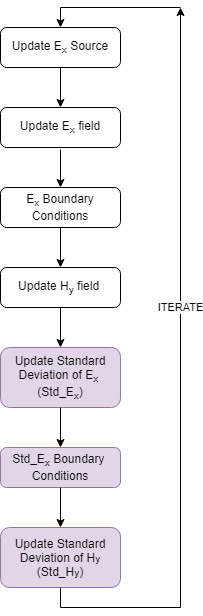
\includegraphics[scale=0.7]{diagramsfdtddef.png}
\caption{FDTD (white) and S-FDTD additions (purple) flow chart \cite{smith2012stochastic}.}
\end{figure}

\section{Mean Field Values}
The delta method \cite{casella2021statistical} will be the tool used to compute the mean and variance of the fields. This method consists on taking a function of stochastic variables and expand it in Taylor's series, next apply the expectation operator and neglect higher order terms getting the following expression for the expectation \cite{smith2012stochastic}:
\begin{equation}
E\lbrace g(x_1,x_2,...,x_n)\rbrace \approx E\lbrace g(\mu_{x_1},\mu_{x_2},...,\mu_{x_n})\rbrace + E \left\lbrace \sum_{i=1}^n \frac{\partial g}{\partial x_i}\bigg |_{\mathrlap{\mu_{x_1},\mu_{x_2}...\mu_{x_n}}}(x_i-\mu_{x_i}) \right\rbrace + ...
\end{equation}
where higher order terms were neglected. Now, using that $E\lbrace x_i\rbrace =\mu_{x_i}$ gives:
\begin{equation}
E\lbrace g(x_1,x_2,...,x_n)\rbrace \approx E\lbrace g(\mu_{x_1},\mu_{x_2},...,\mu_{x_n})\rbrace
\end{equation}
This equation tells us that the expectation of the fields is obtained using the average of the variables in the fields equations \ref{maxwelllossymedium}. Therefore in the S-FDTD method the average of the fields $E_x$ and $H_y$ will be the same as in the traditional FDTD scheme.
\section{Variance of H fields}
For the variance of the fields we start again with the definition:
\begin{equation}
\sigma^2 \lbrace g(x_1,x_2,...,x_n)\rbrace = E\lbrace g(x_1,x_2,...,x_n)^2\rbrace - E\lbrace g(x_1,x_2,...,x_n)\rbrace ^2,
\end{equation}
and now the Taylor expansion is applied obtaining:
\begin{equation}\label{deltamethodvarh}
\sigma^2 \lbrace g(x_1,x_2,...,x_n)\rbrace \approx \sum_{i=1}^n\sum_{j=1}^n \frac{\partial g}{\partial x_i}\frac{\partial g}{\partial x_j} \bigg |_{\mathrlap{\mu_{x_1},\mu_{x_2}...\mu_{x_n}}} E\lbrace(x_i-\mu_{x_i})(x_j-\mu_{x_j})\rbrace,
\end{equation}
where the first term in the expansion of $E\lbrace g(x_1,x_2,...,x_n)^2\rbrace$ cancels out with the expansion of $E\lbrace g(x_1,x_2,...,x_n)\rbrace ^2$ and, again, higher order terms have been neglected.
So the goal is to compute the variance for the updating equation of the $H$ field, for this purpose, two relations involving the variance will be needed, namely:
\begin{equation}\label{Relationsforthevariance}
\begin{split}
\sigma^2\left[X\pm Y\right] & =\sigma_X^2+\sigma_Y^2\pm 2\textit{Cov}(X,Y), \\
\sigma^2\lbrace aX \rbrace  & = a^2 \sigma^2 \lbrace X \rbrace,
\end{split}
\end{equation}
as well as the identity for the covariance $\textit{Cov}(X,Y)=\rho_{XY}\sigma\lbrace X \rbrace \sigma\lbrace Y\rbrace$. \\
\indent The variance of the \textit{H} field equation is:
\begin{equation}
\begin{split}
\sigma^2\left\lbrace H_y^{n+1/2}(k+1/2)-H_y^{n-1/2}(k+1/2)\right\rbrace = \frac{\Delta t^2}{\mu^2 \Delta z^2}\sigma^2\left\lbrace E_x^n(k+1)-E_x^n(k)\right\rbrace
\end{split}.
\end{equation}
This equation can be worked out using the relations \ref{Relationsforthevariance}, getting the result:
\begin{equation}
\begin{split}
& \sigma^2\left\lbrace H_y^{n+1/2}(k+1/2)\right\rbrace-2\sigma\left\lbrace H_y^{n+1/2}(k+1/2)\right\rbrace \sigma\left\lbrace H_y^{n-1/2}(k+1/2)\right\rbrace \\
&+ \sigma^2\left\lbrace H_y^{n+1/2}(k+1/2)\right\rbrace=\frac{\Delta t^2}{\mu^2 \Delta z^2} \left(\sigma^2\left\lbrace E_x^n(k+1)\right\rbrace \right. \\
& \left. -2\sigma\left\lbrace E_x^n(k+1)\right\rbrace \sigma\left\lbrace E_x^n(k)\right\rbrace + \sigma^2 \left\lbrace E_x^n(k)\right\rbrace \right).
\end{split}
\end{equation}
In this equation an approximation has been made, the correlation coefficients have been set equal to one. The correlation coefficient varies between $-1$ and $1$. This coefficient is $\rho_{H_{k+1/2}^{n+1/2},H_{k+1/2}^{n-1/2}}$ for the \textit{H} field, so it is relating the values of the \textit{H} field separated by one time step $\Delta t$ which justifies the approximation. For the correlation coefficient of the \textit{E} field an analogous treatment is made, it's just the correlation between the values of \textit{E} field separated by one spatial step $\Delta z$ \cite{smith2011stochastic}. \\
\indent Observing the last expression for the variance it can be noted that there is a perfect square in each side, taking the square root yields the following update equation for the variance of the \textit{H} field:
\begin{equation}
\sigma\left\lbrace H_y^{n+1/2}(k+1/2) \right\rbrace = \sigma\left\lbrace H_y^{n-1/2}(k+1/2)\right\rbrace + \frac{\Delta t}{\mu \Delta z}\left(\sigma \left\lbrace E_x^n(k+1)\right\rbrace -\sigma\left\lbrace E_x^n(k)\right\rbrace \right).
\end{equation}
It is important to notice that we have to apply the change of variable of the electric field given by equation \ref{changeofvariable} to the latter one when implementing the code. This is a direct computation using the properties of the variance and standard deviation \ref{Relationsforthevariance}.


\section{Variance of E fields}
For the variance of the $E$ field, the same procedure as before is going to be applied. Taking the variance of Ampere's law we get:
\begin{equation}
\begin{gathered}
\sigma^{2}\left\{E_{x}^{n+1}(k)-\frac{\frac{\varepsilon_{r} \varepsilon_{o}}{\Delta t}-\frac{\underline{\sigma}}{2}}{\frac{\varepsilon_{r} \varepsilon_{o}}{\Delta t}+\frac{\underline{\sigma}}{2}} E_{x}^{n}(k)\right\} \\
=\sigma^{2}\left\{\frac { - 1 } { ( \frac { \varepsilon _ { r } \varepsilon _ { 0 } } { \Delta t } + \frac { \underline{\sigma} } { 2 } ) \Delta z } \left(H_{y}^{n+1 / 2}(k+1 / 2) -H_{y}^{n+1 / 2}(k-1 / 2)\right)\right\}.
\end{gathered}
\end{equation}
Now, using the first equation in \ref{Relationsforthevariance} and the relation for the covariance and correlation coefficient, the following expression is obtained
\begin{equation}\label{varecc}
\begin{gathered}
\sigma^{2}\left\{E_{x}^{n+1}(k)-c c E_{x}^{n}(k)\right\}=\sigma^{2}\left\{E_{x}^{n+1}(k)\right\} \\
+\sigma^{2}\left\{c c E_{x}^{n}(k)\right\}-2 \rho_{E E} \sigma\left\{E_{x}^{n+1}(k)\right\} \sigma\left\{c c E_{x}^{n}(k)\right\},
\end{gathered}
\end{equation}
where the next coefficient has been defined:
\begin{equation}
c c=\frac{\frac{\varepsilon_{r} \varepsilon_{o}}{\Delta t}-\frac{\underline{\sigma}}{2}}{\frac{\varepsilon_{r} \varepsilon_{a}}{\Delta t}+\frac{\underline{\sigma}}{2}}.
\end{equation}
The next step is to complete the square in equation \ref{varecc}, this preserves the phases of the variables and will allow a wave-like treatment of the variances analogously to the fields \cite{smith2012stochastic}. Hence, doing this, we get the following expression:
\begin{equation}
\begin{aligned}
&\sigma^{2}\left\{E_{x}^{n+1}(k)-c c E_{x}^{n}(k)\right\} \\
&=\left(\sigma\left\{E_{x}^{n+1}(k)\right\}-\rho_{E E} \sigma\left\{c c E_{x}^{n}(k)\right\}\right)^{2} \\
&\quad+\left(1-\rho_{E E}^{2}\right) \sigma^{2}\left\{c c E_{x}^{n}(k)\right\},
\end{aligned}
\end{equation}
with $\rho_{E E}=\rho_{E_x^{n+1}(k),cc E_x^{n}(k)}$, and this correlation coefficient is assumed to be one \cite{smith2011stochastic}. After this, the last equation simplifies to 
\begin{equation}
\sigma^{2}\left\{E_{x}^{n+1}(k)-c c E_{x}^{n}(k)\right\} \approx \left(\sigma\left\{E_{x}^{n+1}(k)\right\}- \sigma\left\{c c E_{x}^{n}(k)\right\}\right)^{2}.
\end{equation}
\indent From this equation, a series of approximations and some algebra are used to derive the equation for the variance of the $E$ field. The first thing is to expand the second term of the right hand side, to this purpose the delta method, namely equation \ref{deltamethodvarh}, is employed. The algebra is cumbersome as nine terms show up, in this case the function is $g\left(\epsilon_r, \underline{\sigma}, E_x^n\right)=cc E_x^n$. Some terms are somehow easy to get, for example, the term of 
\begin{equation}
\frac{\partial g}{\partial E_x^n} \frac{\partial g}{\partial E_x^n} \bigg |_{\mathrlap{\mu_{\epsilon_r}, \mu_{\underline{\sigma}}}} E\{(E_x^n-\mu_{E_x^n})(E_x^n-\mu_{E_x^n})\}=\frac{\left(2 \varepsilon_{o} \mu_{\varepsilon_{r}}-\Delta t \mu_{\underline{\sigma}}\right)^{2}}{\left(2 \varepsilon_{o} \mu_{\varepsilon_{r}}+\Delta t \mu_{\underline{\sigma}}\right)^{2}} \sigma^{2}\left\{E_{x}^{n}(k)\right\}.
\end{equation}
After some algebra, the variance equation for the electric field can be expressed as:
\begin{equation}\label{stde}
\begin{aligned}
&\sigma\left\{E_{x}^{n+1}(k)\right\} \approx \frac{2 \varepsilon_{o} \mu_{\varepsilon_{r}}-\Delta t \mu_{\underline{\sigma}}}{2 \varepsilon_{o} \mu_{\varepsilon_{r}}+\Delta t \mu_{\underline{\sigma}}} \sigma\left\{E_{x}^{n}(k)\right\} \\
&+\frac{2 \Delta t}{\Delta z\left(2 \varepsilon_{o} \mu_{\varepsilon_{r}}+\Delta t \mu_{\underline{\sigma}}\right)}\left(\begin{array}{c}
\sigma\left\{H_{y}^{n+1 / 2}(k+1 / 2)\right\} \\
-\sigma\left\{H_{y}^{n+1 / 2}(k-1 / 2)\right\}
\end{array}\right) \\
\quad & +\frac{4 \Delta t \varepsilon_{o}\left(\mu_{\underline{\sigma}} \rho_{\varepsilon_{r}, E} \sigma\left\{\varepsilon_{r}\right\}-\mu_{\varepsilon_{r}} \rho_{\underline{\sigma}, E} \sigma\{\underline{\sigma}\}\right)}{\left(2 \varepsilon_{o} \mu_{\varepsilon_{r}}+\Delta t \mu_{\underline{\sigma}}\right)^{2}} E_{x}^{n}(k) \\
&-\frac{2 \Delta t}{\Delta z\left(2 \varepsilon_{o} \mu_{\varepsilon_{r}}+\Delta t \mu_{\underline{\sigma}}\right)} 
\cdot\left(\begin{array}{c}
\frac{\left(2 \varepsilon_{o} \sigma\left\{\varepsilon_{r}\right\} \rho_{\varepsilon_{r}, H_{y}^{n+1 / 2}}+\Delta t \sigma\{\underline{\sigma}\} \rho_{\underline{\sigma}, H_{y}^{n+1 / 2}}\right)}{\left(2 \varepsilon_{o} \mu_{\varepsilon_{r}}+\Delta t \mu_{\underline{\sigma}}\right)} \\
\cdot \left(H_{y}^{n+1 / 2}(k-1 / 2)-H_{y}^{n+1 / 2}(k+1 / 2)\right)
\end{array}\right).
\end{aligned}
\end{equation}
\indent As mentioned before for the case of the variance for the $H$ field, the change of variable \ref{changeofvariable} must be applied to this equation as well. Now, we have almost finished the derivation of the S-FDTD method. The only thing left are the boundary conditions for the variance fields. Variances exhibit an analogous behavior to the mean fields computed with the FDTD and thus require boundary conditions. The same absorbing conditions will be applied in this case, it suffices with replacing the electric fields with their standard deviation in equations \ref{boundarycondition1} and \ref{boundarycondition2}. \\
\indent The biggest issue with equation \ref{stde} is that, in principle, we do not know much about the four correlation coefficients that are present. Of course, they are bounded between $-1$ and $1$. Different approximations have been tried in the literature as it will be explored later. For example, setting the coefficients equal to one has been found to overestimate the variance given  by the Monte Carlo method.


\section{Standard Deviation in Reflectance and Transmittance.}\label{stdRsection}
With the previous formalism, it has been possible to obtain the standard deviation of the fields. Now, the standard deviation of the reflection and transmission coefficient is sought. To perform this task, the propagation of errors is going to be employed. Let consider the reflectance, which expression is:
\begin{equation}
R=\frac{|E_{reflected}(\omega)|}{|E_{source}(\omega)|} ,
\end{equation}
where the source field has no standard deviation and can be treated as a constant. Now, the standard deviation of $R$ is:
\begin{equation}\label{sigmaR1}
\sigma\{R\}= \frac{\partial R}{\partial |E_{ref}(\omega)|} \sigma\{|E_{ref}(\omega)|\}.
\end{equation}
\indent On the other hand, given a quantity $X$, which is a function of other variables $X=f(x_1,x_2,...)$, the variance of $X$, in case $f$ is a linear combination of the variables $\left( f= \sum_i^n a_i x_i \right)$, is \cite{taylor1997introduction}: 
\begin{equation}\label{errorpropagationvariance}
\sigma_X ^2 = \sum_i ^n a_i^2 \sigma_i^2 + \sum_i^n \sum_{j(j\neq i)} ^n a_i a_j \rho_{ij} \sigma_i \sigma_j,
\end{equation}
and this is the case at hand since $E_{ref}(\omega)$ was obtained using the discrete Fourier transform (DFT), which is a linear combination of the electric fields in time space:
\begin{equation}
E_k(\omega)=\sum_{n=0}^{N-1} e^{-i\frac{2\pi}{N} k n} E^n(t).
\end{equation} 
The coefficients of the Fourier transform can be identified with the $a's$ in \ref{errorpropagationvariance}, where the second term is the covariance written in terms of the correlations $\rho_{ij}$. In the S-FDTD formalism the correlations between electric fields at different times is high and it is assumed to be one \cite{smith2011stochastic}. Using this, expression \ref{errorpropagationvariance} can be written as a perfect square (multinomial theorem):
\begin{equation}
\sigma_X=\sum_i ^n a_i \sigma_i.
\end{equation}
Now, this last equation means that $\sigma\{E_{ref}(\omega)\}$ can be obtained applying the Fourier transform to the standard deviation of the fields (the outputs of S-FDTD scheme). \\
\indent From now on, a procedure that will not be proved is carried out. Although no proof is provided and no information has been found in the literature, the following result is validated in the results section. \\
\indent The idea behind the next step is to assign the real part of the standard deviation of the fields to the real part of the fields and to do the same with the imaginary parts. Doing this, the error propagation expression can be written in the following way:
\begin{equation}
\sigma\{|E_{ref}(\omega)|\}=\frac{\Re{(E_{ref}(\omega))}}{|E_{ref}(\omega)|} \cdot \Re{(\sigma\{E_{ref}(\omega)\})} + \frac{\Im{(E_{ref}(\omega))}}{|E_{ref}(\omega)|} \cdot \Im{(\sigma\{E_{ref}(\omega)\})}
\end{equation}
The last step is just to use this expression in equation \ref{sigmaR1} which gives 
\begin{equation}
\sigma\{R\}=\frac{1}{|E_{source}(\omega)|}\sigma\{|E_{ref}(\omega)|\}
\end{equation}
The equation for the transmission coefficient is obtained in an analogous way.

\chapter{Monte Carlo FDTD.}
\section{Introduction to the M-FDTD method.}
\indent Monte Carlo method \cite{Hastings1995,Ajayi2008} is the traditional approach to evaluate statistical quantities such as the mean and variance. This method is well known and widely used in several areas of physics. In the case at hand, the Monte Carlo is applied to the usual FDTD algorithm explained before. \\
\indent The M-FDTD algorithm will be used to compare the results obtained with the S-FDTD. The differences will depend mainly in the choice of the correlation coefficients in the S-FDTD variance equations, therefore the Monte Carlo can be used to check the validity of a particular choice or even to estimate the value of the correlations \cite{Bisheh2015}. \\
\indent The first step for the M-FDTD is to generate the parameters, namely the permittivity and conductivity, randomly distributed according to a given distribution. The Gaussian distribution have been chosen for the main results although other distributions could be used to produce the electrical parameters, for this purpose the Metropolis algorithm can be employed. Variability could also be introduced in the thickness of the materials but this will not be approached in this work. \\
\indent Variability can be present in materials for several reasons. Consider some inhomogeneous materials such as biological tissues like skin, fat or muscle. The composition and therefore the electrical properties will vary among people, for example, tissues' conductivities will depend on the level of hydration of the individual.
Another way in which variability can appear is due to measurement uncertainties. Although variability starts in the materials due to these uncertainties, it will propagate to the air layer, which has not variability. This is explained due to the reflected fields which carry this variability to the air. \\
\indent In the next sections, two different schemes for computing the Monte Carlo will be explored to treat the two sources of uncertainties explained here. 

\section{Scheme of the Monte Carlo method.}
\indent The Monte Carlo will perform a lot of FDTD simulations with random parameters. After every simulation is run, the quantities of interest are recorded. In this study, the electric field at every cell in the mesh and the reflectance and transmittance were added in some variables while the simulations were running. At the end of the simulations, the following equations allow us to obtain the mean and standard deviation:
\begin{equation}\label{mean_mc}
\mu_X=\frac{1}{N} \sum_{i=1}^N x_i,
\end{equation}
\begin{equation}\label{std_mc1}
\sigma_X=\sqrt{\frac{1}{N-1}  \sum_{i=1}^N \left(x_i-\mu_X \right)^2}.
\end{equation}
In the equation for the mean \ref{mean_mc}, the summation was computed during the simulations, so the only step left is to divide by $N$, the number of FDTD simulations. The equation for the standard deviation in the form of \ref{std_mc1} does not allow us to compute it directly while the simulations are running because the mean remains unknown until all the simulations are performed, however this expression can be rewritten in the following manner
\begin{equation}
\sigma_X=\sqrt{\frac{1}{N-1} \left( \left[ \sum_{i=1}^N x_i^2  \right] - N\mu_X^2 \right)}.
\end{equation}
Now, the summation in this equation can be performed meanwhile the FDTD simulations so that the values $x_i$ need not to be stored. \\
\indent There are more statistical quantities that can be computed and the most important one in this context is the correlation coefficient. Correlation coefficients appear in the one of the equations obtained using the S-FDTD method, the expression for the standard deviation of the electric field \ref{stde}. Using the next equations those can be computed:
\begin{equation}
Cov_{X,Y}=\frac{1}{N-1} \sum_{i=1}^N \left(x_i-\mu_X\right)\left(y_i-\mu_Y\right),
\end{equation}
\begin{equation}
\rho_{X,Y}=\frac{Cov_{X,Y}}{\sigma_X \sigma_Y}.
\end{equation}
Using the last equation we can compare the results of the Monte Carlo method for correlation coefficients with our previous choice of those in the S-FDTD scheme. Furthermore, the M-FDTD method can be used to estimate this coefficients which will then be used in the S-FDTD. This only have sense if a small number of runs is performed using the Monte Carlo, as running it many times will get the statistical parameters of interest, hence there will be no need to use the S-FDTD. The correlation coefficients that appear in the S-FDTD formalism are $\rho_{\bar{\sigma},E^n},\rho_{\epsilon_r,E^n},\rho_{\bar{\sigma},H^{n+1/2}},\rho_{\epsilon_r,H^{n+1/2}}$, and are time dependent. Using the method proposed to estimate them it is found that only the value at a certain time step is needed to obtain significant results \cite{Bisheh2015}.

\section{Understanding randomness in electrical parameters.}
In the simulations run with the code developed for this work some peculiar results have been found. The first step to perform the Monte Carlo simulation was to generate the normal distributed random parameters for the electrical properties. \\
\indent The first approach (``layer by layer") tried treated every layer in the set of materials as a whole, hence, given the permittivity and conductivity of each material, an array of dimension equal to the number of simulations was built with each element being the random parameter for this material. In other words, a number of materials equal to the number of simulations was generated. This method reproduce the results found in \cite{smith2011stochastic} for the variance but does not approximate well to the S-FDTD method for reproducing the reflectance and transmittance. \\
\indent To solve the issues mentioned in the last paragraph the materials were treated ``cell by cell". In this case, each cell belonging to each layer is assigned a random parameter following the same distribution as before. With this approach, the problem that occurs in the reflectance and transmittance was solved, but the variance of the electric fields differs from the results presented in \cite{smith2011stochastic}. This will be treated in the results section. This formalism looks convenient when we are treating an inhomogeneous material.

\chapter{Results.}
In this section, the different methods will be validated and compared amid them and with the results found in the literature \cite{smith2011stochastic}.

\section{Validation of the FDTD method.}
This section is devoted to the validation of the first method which is also the base for the S-FDTD formalism. Three graphs for the reflection and transmission coefficients are presented, they are obtained following the procedure of section \ref{rytfromthesfdtdscheme}. In Figure \ref{r2+t2=1} it can be observed that the reflectance and transmittance sum up to one in agreement with \ref{r2+t21}. The material chosen for this simulation had a thickness of $d=3\text{cm}$ with a relative permittivity $\epsilon_r=4$ and no conductivity.\\
\indent The next result of this section (Figure \ref{rytvspanel}) is obtained using the same material, but this time the conductivity was set to $\sigma=0.04 \text{S/m}$. Now, this is a lossy dielectric medium and relation \ref{r2+t21} will not hold. In this graph the analytic result \ref{analyticresultrt} is superimposed on the FDTD result and is almost indistinguishable in that frequency range. \\
\indent For the last representation (Figure \ref{rytvspanel3materiales}), the goal is to check expression \ref{variosmateriales}. The materials' parameters, here and for the rest of the results section, are those shown in Figure \ref{parameterstable}. Again, the agreement amid the analytic result and the FDTD is achieved so the expression mentioned is checked.

\begin{figure}
\centering
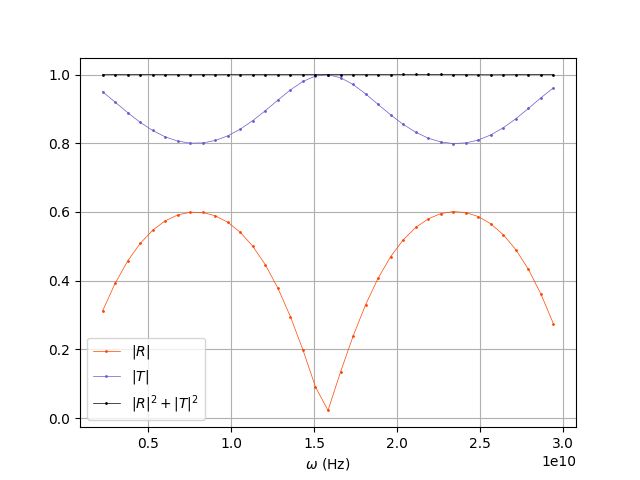
\includegraphics[scale=0.7]{rytlosslessmedium(1).png}
\caption{Reflectance and transmittance for a lossless medium.}\label{r2+t2=1}
\end{figure}

\begin{figure}
\centering
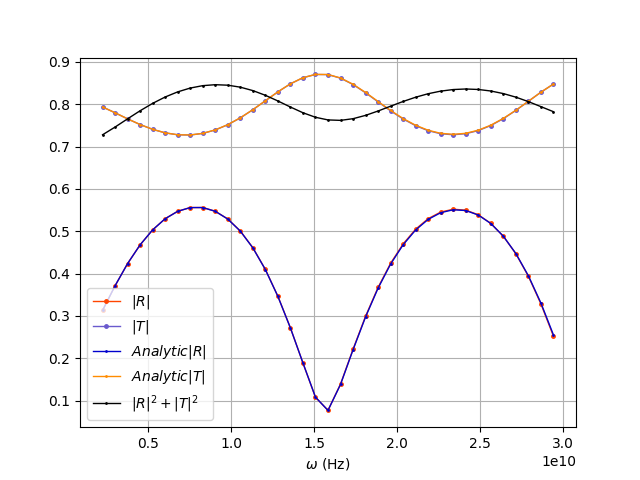
\includegraphics[scale=0.7]{rytvspanel(2).png}
\caption{Reflectance and transmittance for a lossy dielectric medium.}\label{rytvspanel}
\end{figure}

\begin{figure}
\centering
\includegraphics[scale=0.7]{parameterstable.png}
\caption{Electrical parameters for the biological tissues used in this section. This data is taken from \cite{smith2012stochastic}, which allow for a comparison of the results.}\label{parameterstable}
\end{figure}

\begin{figure}
\centering
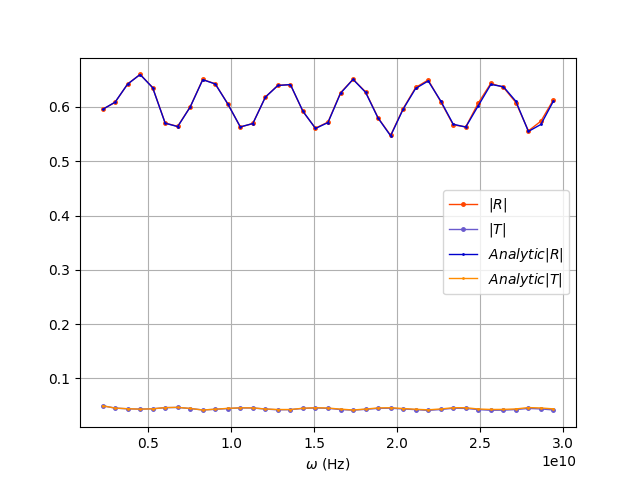
\includegraphics[scale=0.7]{rytvspanel3materiales(3).png}
\caption{Reflectance and transmittance for a lossy dielectric medium with three materials.}\label{rytvspanel3materiales}
\end{figure}

\section{Validation of the S-FDTD formalism.}
Now, a validation of the method explained in section \ref{stdRsection} is sought. The procedure explained there enables us to compute the standard deviation of the reflection and transmission coefficients. To validate this, a plot of the reflection coefficient with errorbars is presented. The errorbars are the standard deviation of this coefficient. Within this same figure (\ref{stdRgauss(4)}), there are two more quantities, they are the reflection coefficient obtained with the average field value plus and minus the standard deviation. It can be seen that these values reach the maximum and minimum value of the errorbars respectively, hence validating this way of computing the standard deviation of the reflection and transmission coefficients. The same plot is repeated using a sinusoidal source instead of the Gaussian pulse (Figure \ref{stdR(5)}). \\
\indent The next thing which is going to be shown are the plots of these coefficients with the corresponding errorbars, obtained with the S-FDTD method for two different values of the correlation coefficients of equation \ref{stde}, versus the coefficients obtained with each one of the two Monte Carlo variations discussed before. The Monte Carlo method is run for $10000$ single FDTD simulations in all cases from now on. In Figure \ref{stdR(6)} it can be seen that the ``layer by layer" Monte Carlo, which is the one used in references \cite{smith2011stochastic,smith2012stochastic}, does not reproduce well the average value of the reflection coefficient. The S-FDTD  is able to perform this task as was checked before with the analytical result. This also happens if the source is the one used in the literature, namely, the sinusoidal source (Figure \ref{stdR(10)}). Now, we can compare these two last plots with the other approach for the Monte Carlo, i.e. the ``cell by cell" Monte Carlo method. In this case, the result given by the Monte Carlo is able to reproduce the analytic one for the average value of the reflection and transmission coefficients (see Figures \ref{stdR(8)} and \ref{stdR(11)}). The same behavior is found for the transmission one (Figures \ref{stdT(7)} and \ref{stdT(9)}). \\
\indent Lastly, a plot is presented (Figure \ref{stdRcorr05(8)})  to see the effect of the change in the correlation coefficients in equation \ref{stde}. With all the correlations set equal to $0.5$, it can be seen that the errorbars are significant lower in magnitude compared with those obtained for the correlations equal to one.

\begin{figure}
\centering
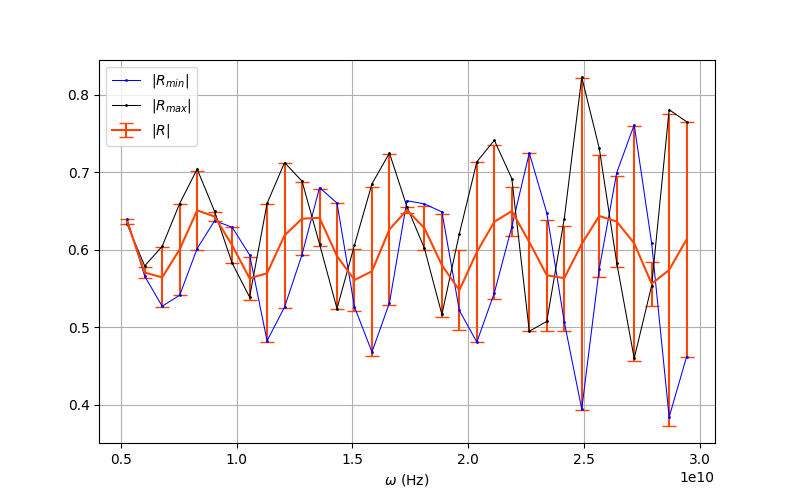
\includegraphics[scale=0.7]{stdRgauss(4).png}
\caption{Validation of the procedure used to compute the standard deviation of the reflection and transmission coefficients (Gaussian pulse source). The extremes of the errorbars match the two reflection coefficients computed using $E+\sigma(E)$ and $E-\sigma(E)$.}\label{stdRgauss(4)}
\end{figure}

\begin{figure}
\centering
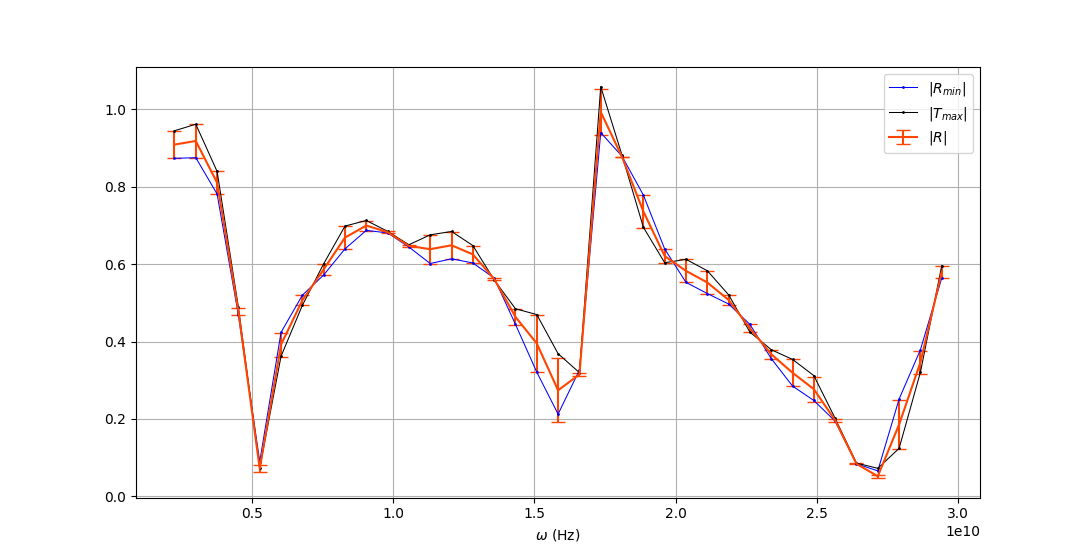
\includegraphics[scale=0.55]{stdRsin(5).png}
\caption{Validation of the procedure used to compute the standard deviation of the reflection and transmission coefficients (Sinusoidal source).}\label{stdR(5)}
\end{figure}

\begin{figure}
\centering
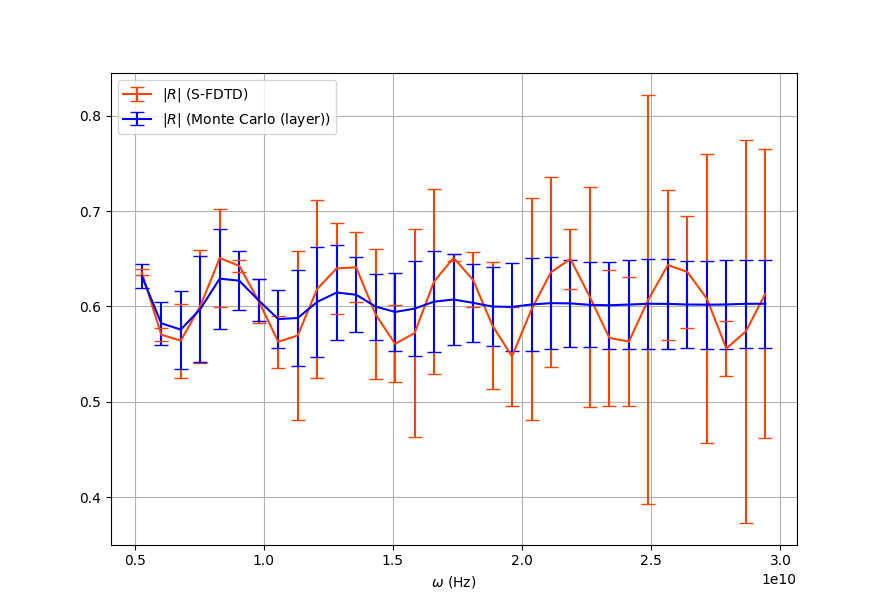
\includegraphics[scale=0.5]{Rsfdtdmcgausslayercorr1(6).png}
\caption{Reflection coefficient for all correlation coefficients set equal to one (S-FDTD). For the Monte Carlo method, the first approach is selected (``layer by layer").}\label{stdR(6)}
\end{figure}

\begin{figure}
\centering
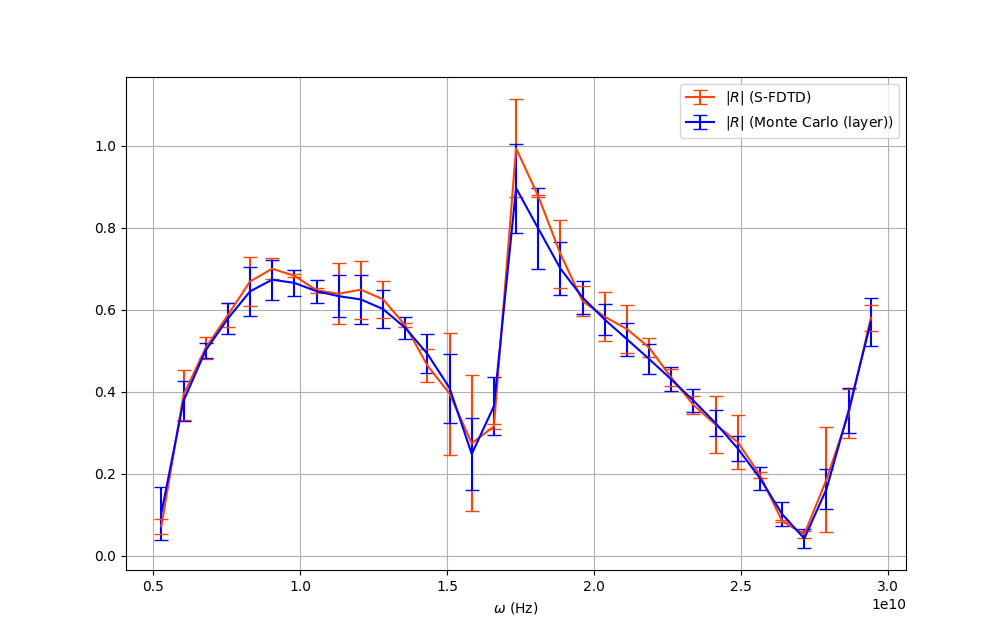
\includegraphics[scale=0.5]{Rsfdtdmcsinlayer(10).png}
\caption{Reflection coefficient for all correlation coefficients set equal to one (S-FDTD). For the Monte Carlo method, the first approach is selected (``layer by layer") with a sinusoidal source.}\label{stdR(10)}
\end{figure}

\begin{figure}
\centering
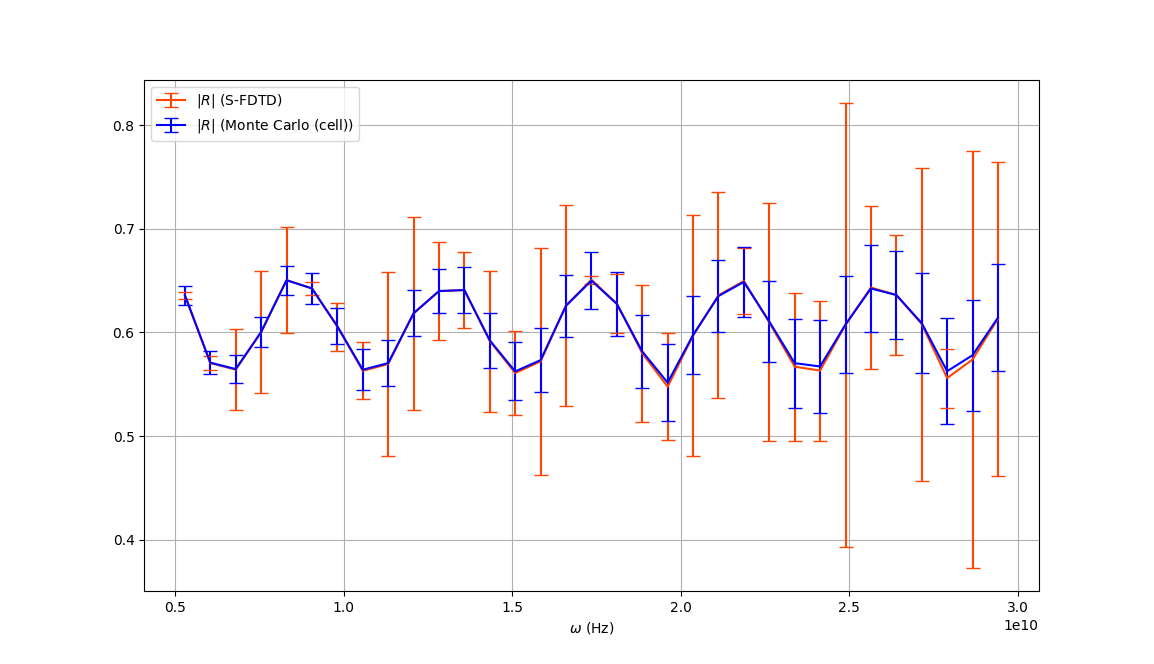
\includegraphics[scale=0.48]{Rsfdtdmcgausscellcorr1(8).png}
\caption{Reflection coefficient for all correlation coefficients set equal to one (S-FDTD). For the Monte Carlo method, the second approach is selected (``cell by cell") with a Gaussian pulse as the source.}\label{stdR(8)}
\end{figure}

\begin{figure}
\centering
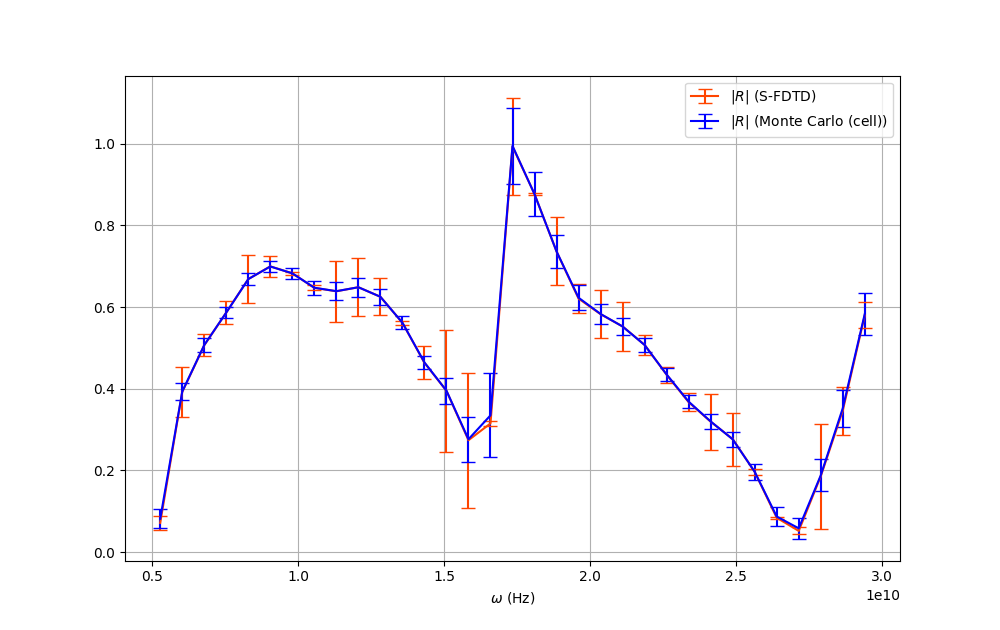
\includegraphics[scale=0.48]{Rsfdtdmcsincell(11).png}
\caption{Reflection coefficient for all correlation coefficients set equal to one (S-FDTD). For the Monte Carlo method, the second approach is selected (``cell by cell") with a sinusoidal source.}\label{stdR(11)}
\end{figure}

\begin{figure}
\centering
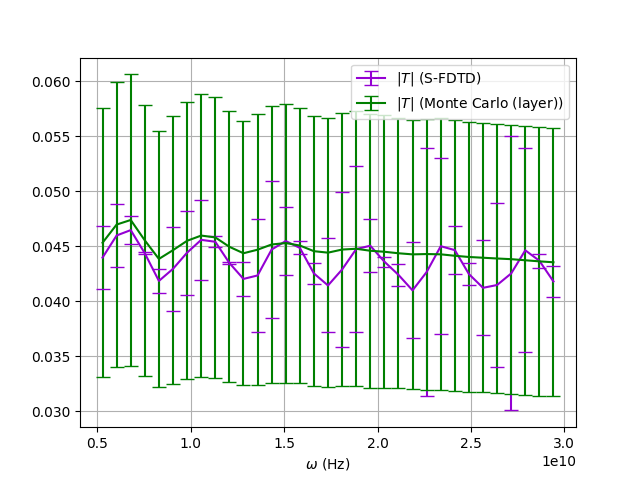
\includegraphics[scale=0.65]{Tsfdtdmcgausslayercorr1(7).png}
\caption{Transmission coefficient. For the Monte Carlo method, the second approach is selected (``layer by layer") with a Gaussian pulse as the source.}\label{stdT(7)}
\end{figure}

\begin{figure}
\centering
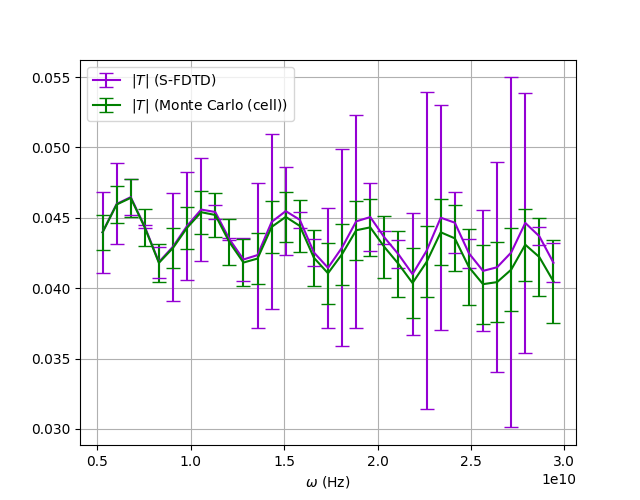
\includegraphics[scale=0.65]{Tsfdtdmcgausscellcorr1(9).png}
\caption{Transmission coefficient. For the Monte Carlo method, the second approach is selected (``cell by cell") with a Gaussian pulse as the source.}\label{stdT(9)}
\end{figure}

\begin{figure}
\centering
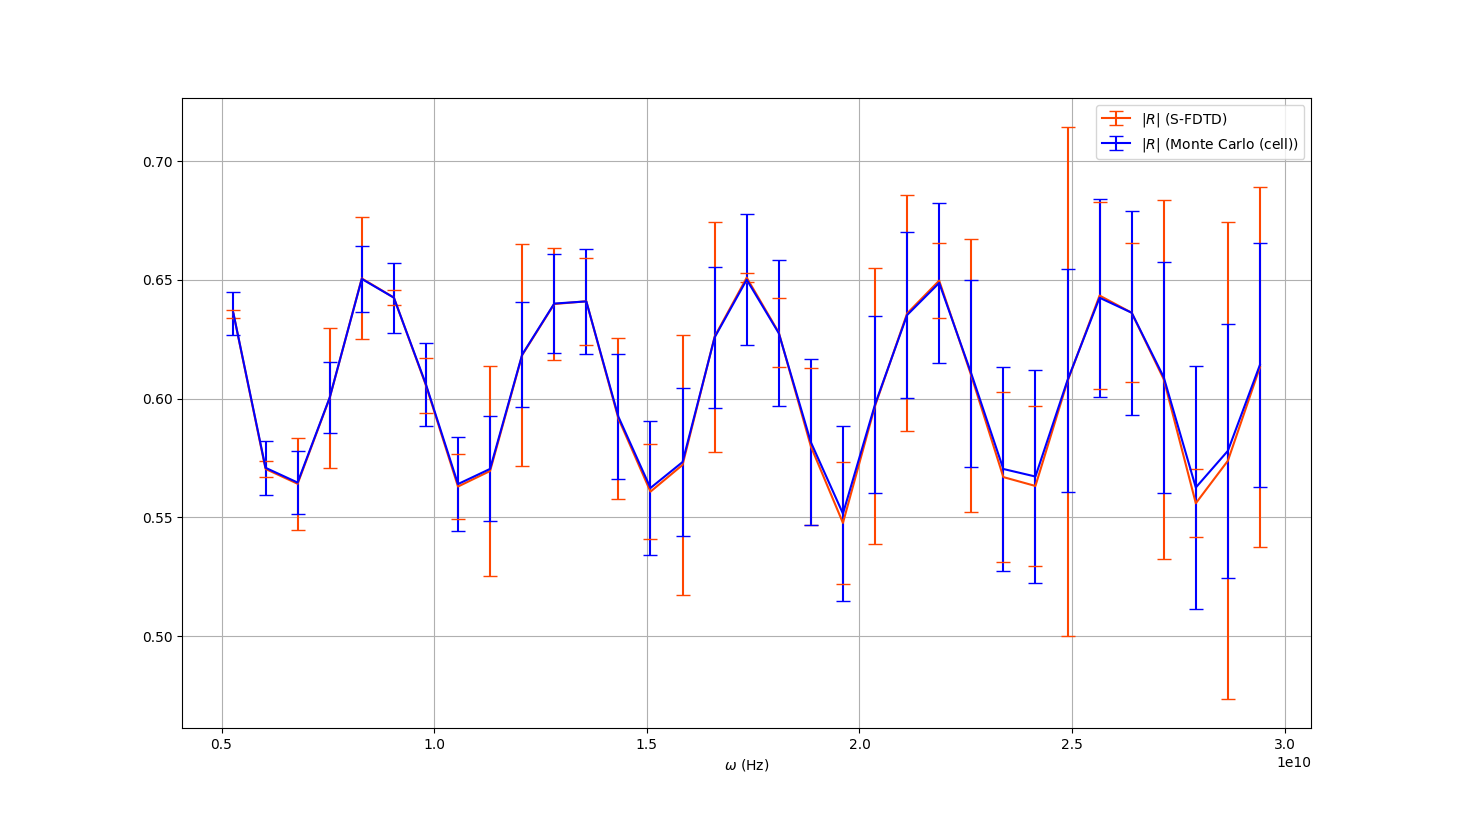
\includegraphics[scale=0.4]{Rsfdtdmcgausscellcorr05(8).png}
\caption{Reflection coefficient with all correlation coefficients set equal to $0.5$. For the Monte Carlo method, the second approach is selected (``cell by cell") with a Gaussian pulse as the source.}\label{stdRcorr05(8)}
\end{figure}

\section{Snapshots of the average fields and the variance}
Here, four plots are included, they are snapshots of the $10000$ time step of the simulations. Two of them represent the average values for the two Monte Carlo methods. Again, the Monte Carlo ``layer by layer" fails to reproduce the average values whereas with this method we are able to get the results for the variance found in \cite{smith2011stochastic,smith2012stochastic}. On the other hand, the ``cell by cell" approach get the same result as the FDTD for the average values, it is indistinguishable from the plot, but obtain a significant lower variance that the one showed in \cite{smith2012stochastic} (see Figures from \ref{Exlayer(12)}).

\begin{figure}
\centering
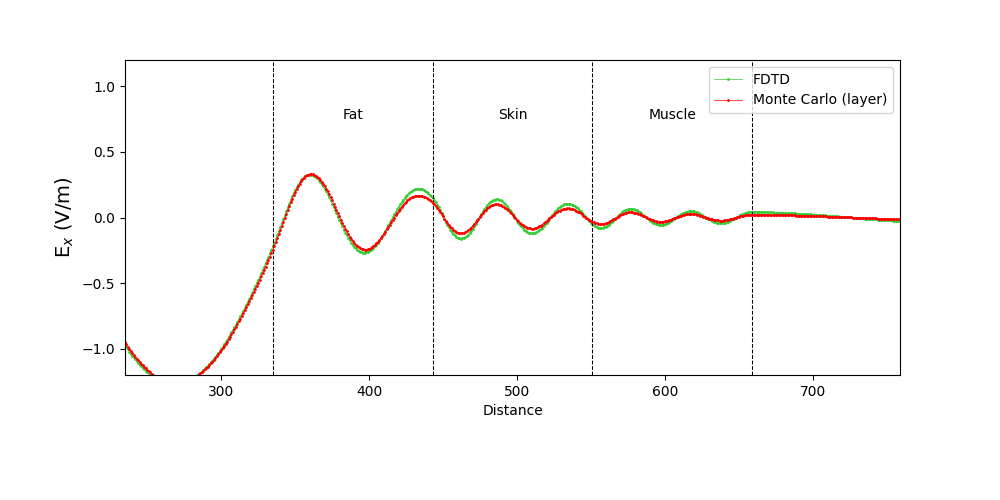
\includegraphics[scale=0.6]{Exlayer(12).png}
\caption{Snapshot for the average field values. The approach used in the Monte Carlo method is the ``layer by layer" one. The distance is given by the cell number of the mesh.}\label{Exlayer(12)}
\end{figure}

\begin{figure}
\centering
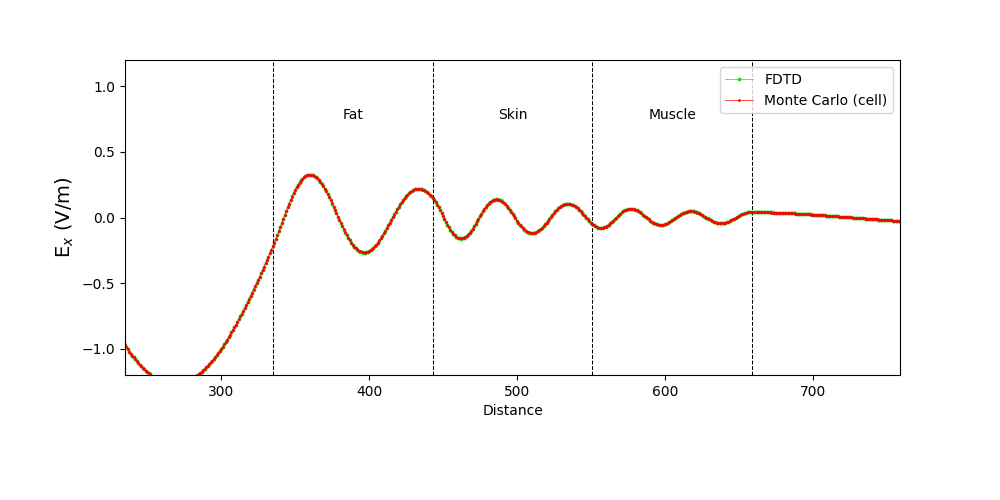
\includegraphics[scale=0.6]{Excell(14).png}
\caption{Snapshot for the average field values. The approach used in the Monte Carlo method is the ``cell by cell" one.}\label{Excell(14)}
\end{figure}


\begin{figure}
\centering
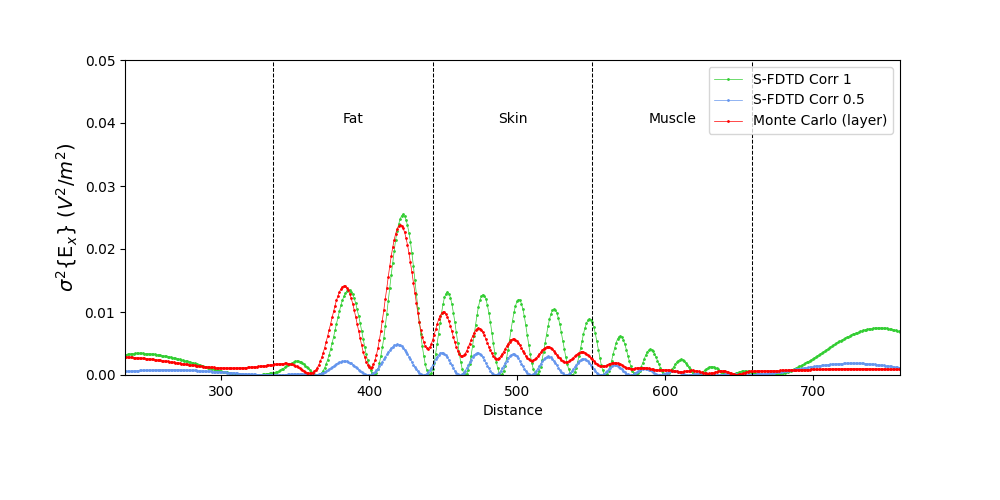
\includegraphics[scale=0.6]{Vaexlayer(13).png}
\caption{Snapshot for the variance of the fields. The approach used in the Monte Carlo method is the ``layer by layer" one.}\label{VarExlayer(13)}
\end{figure}


\begin{figure}
\centering
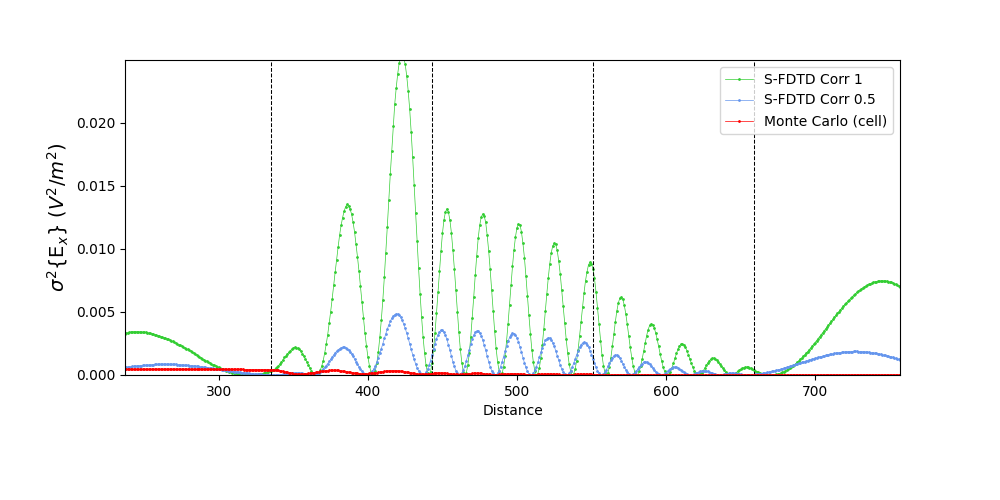
\includegraphics[scale=0.6]{VarExcell(15).png}
\caption{Snapshot for the variance of the fields. The approach used in the Monte Carlo method is the ``cell by cell" one.}\label{VarExcell(15)}
\end{figure}

\chapter{Conclusions.}
In this work a review of the FDTD method has been done. With this previous formalism in mind was possible to extend it and add the two equations for the standard deviation of the fields. \\
\indent At this point, the need of obtaining the standard deviation of the reflection and transmission coefficients was one of the main problems found. A procedure to obtain these standard deviations was derived and, although it was not proved, has been validated in the results section. \\
\indent The next step was to implement the Monte Carlo method, but following the most intuitive approach, this is, to consider each material layer as a whole resulted in great disagreement when computing the reflectance and transmittance. Furthermore, this method, which is the one used in the referenced literature, is not capable of reproducing the average values of the fields either. To give an answer to these issues, another proposal of making the Monte Carlo simulations was sought. This new approach can be thought as if the material layers were discretized and each point is treated randomly. With this method the disagreement in the reflection and transmission coefficients was solved, however the variance of the fields was found to be significant lower compared with the previous method. \\
\indent The discussion made in the last paragraph about how the materials should be treated must be connected to the nature of the uncertainties. If we are considering an inhomogeneous  material, in which each part of his volume differs from other parts, it makes sense to treat this material ``cell by cell" or ``point by point". On the other hand, if the cause is the uncertainty in the measurement, the other approach seems more suitable. \\








%\chapter{Los enunciados}

%\section{Teoremas y demostraciones}


%\begin{theorem}[Euclides]\label{thm:th1}
   % Esto es un Teorema. Se numeran a partir del 1 en cada capítulo. Como son importantes, %tienen un cuadrado rojo al principio. Llevan letra cursiva.
%\end{theorem}

%\begin{proof}
%    Esto es la demostración. Al final de la demostración se puede ver un cuadrado rojo %similar al de los teoremas. Las demostraciones no llevan letra cursiva.
%\end{proof}


%\begin{definition}\label{def:1}
%    Esto es una definición. Las definiciones son importantes; también llevan un %cuadradito rojo.
%\end{definition}


%\subsection{Otros enunciados}


%\begin{remark}
%    Esto es una observación, que dice que $e=mc^{2}$. Como las observaciones no son %importantes, no llevan cuadrado rojo, y el tipo de letra no es cursiva.
%\end{remark}


%\begin{proof}
    %Si la demostración acaba en una fórmula, para poner el cuadrado rojo a la altura de %la última formula, hay que usar la orden \verb|\qedhere|, como en este caso:
%    \[
%        e=mc^{2}.\qedhere
%   \]

%\end{proof}


%\begin{corollary}\label{cor:1}
  %  Esto es un corolario.
%\end{corollary}

%\begin{proposition}\label{pro:1}
%   Esto es una proposición.
%\end{proposition}

%\begin{lemma}[Gauss]\label{lem:1}
    %Esto es un lema.
%\end{lemma}


%\backmatter

\bibliographystyle{ieeetr}
\nocite{*}
\bibliography{tfm} % -> lee miarchivo.bib
%===============


\end{document}